\section{A Plataforma VIDA}
\label{sec:plataforma}

O Veículo Inteligente de Desenvolvimento Aplicado (VIDA) é uma plataforma experimental de pequeno porte, desenvolvida pelo Laboratório de Mobilidade Terrestre (LMT), da Universidade Federal de Lavras (UFLA). Iniciado em 2019, o projeto tem como finalidade disponibilizar um veículo elétrico para o desenvolvimento, a integração e a validação de tecnologias relacionadas à condução autônoma. 

A plataforma foi concebida para apoiar pesquisas nas áreas de instrumentação, localização, navegação e controle de veículos terrestres. Sua utilização permite avaliar algoritmos e sistemas embarcados em condições reais de operação, contribuindo para a aproximação entre o desenvolvimento teórico e a validação experimental. 

A Figura~\ref{fig:vida_atual} apresenta a plataforma VIDA em sua configuração atual, utilizada neste trabalho.

\begin{figure}[htb]
    \centering
    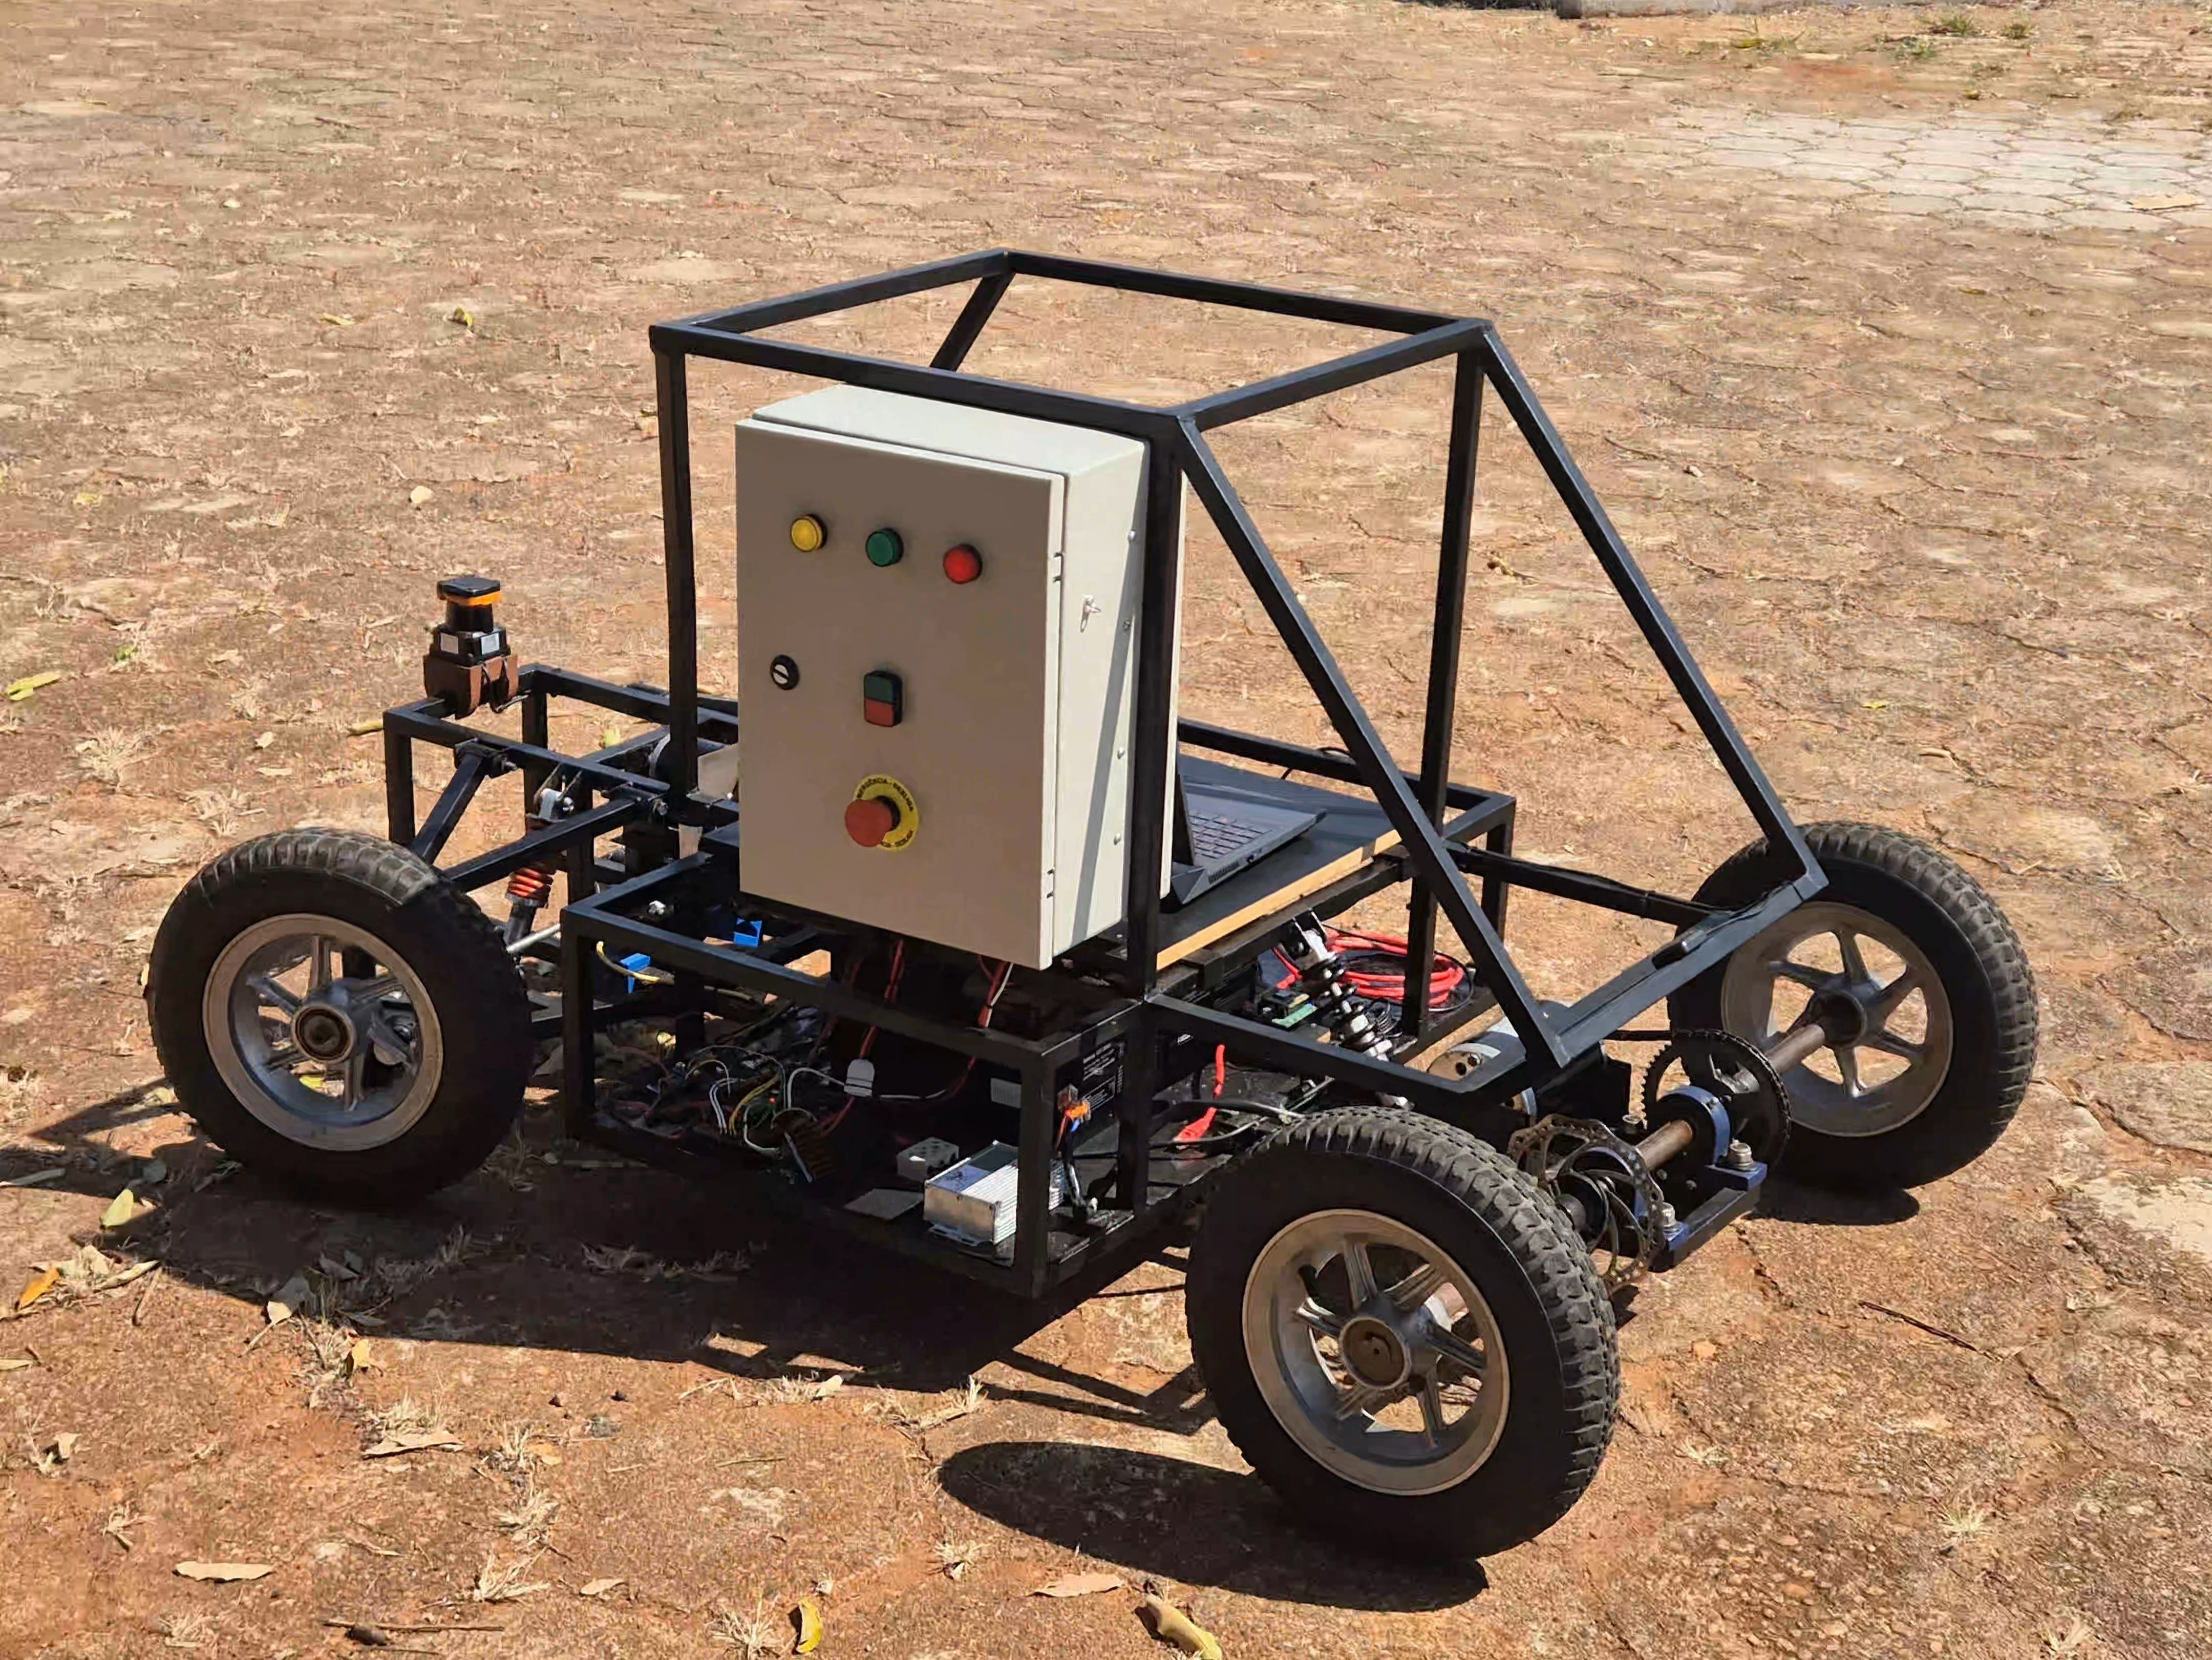
\includegraphics[width=0.72\columnwidth]{Imagens/Vida 1.jpg}
   \caption{Estado atual da plataforma VIDA. Fonte: Acervo do autor.}
    \label{fig:vida_atual}
\end{figure}

\subsection{Estrutura Mecânica}

A estrutura mecânica do VIDA foi desenvolvida em etapas anteriores do projeto, sendo constituída por um chassi metálico modular, com quatro rodas, tração traseira e esterçamento nas rodas dianteiras. Essa configuração permite a instalação de diferentes componentes e instrumentos, conforme as necessidades das pesquisas desenvolvidas na plataforma. 

Durante a evolução do projeto, a estrutura do veículo recebeu modificações, destacando-se a instalação de um suporte metálico elevado, desenvolvido por \citet{Lorenzato2026}. Essa estrutura foi projetada para acomodar câmeras de visão estéreo e permitir o posicionamento do receptor GNSS em relação ao eixo traseiro do veículo.

O sistema de esterçamento também passou por uma modificação, realizada no âmbito das atividades deste trabalho, envolvendo o redimensionamento do motor elétrico e a modificação do conjunto de transmissão mecânica. O novo mecanismo utiliza polias e correia dentada para transmitir o movimento do motor ao sistema de direção, conforme apresentado na Figura~\ref{fig:estercamento_vida}.

\begin{figure}[htb]
    \centering
    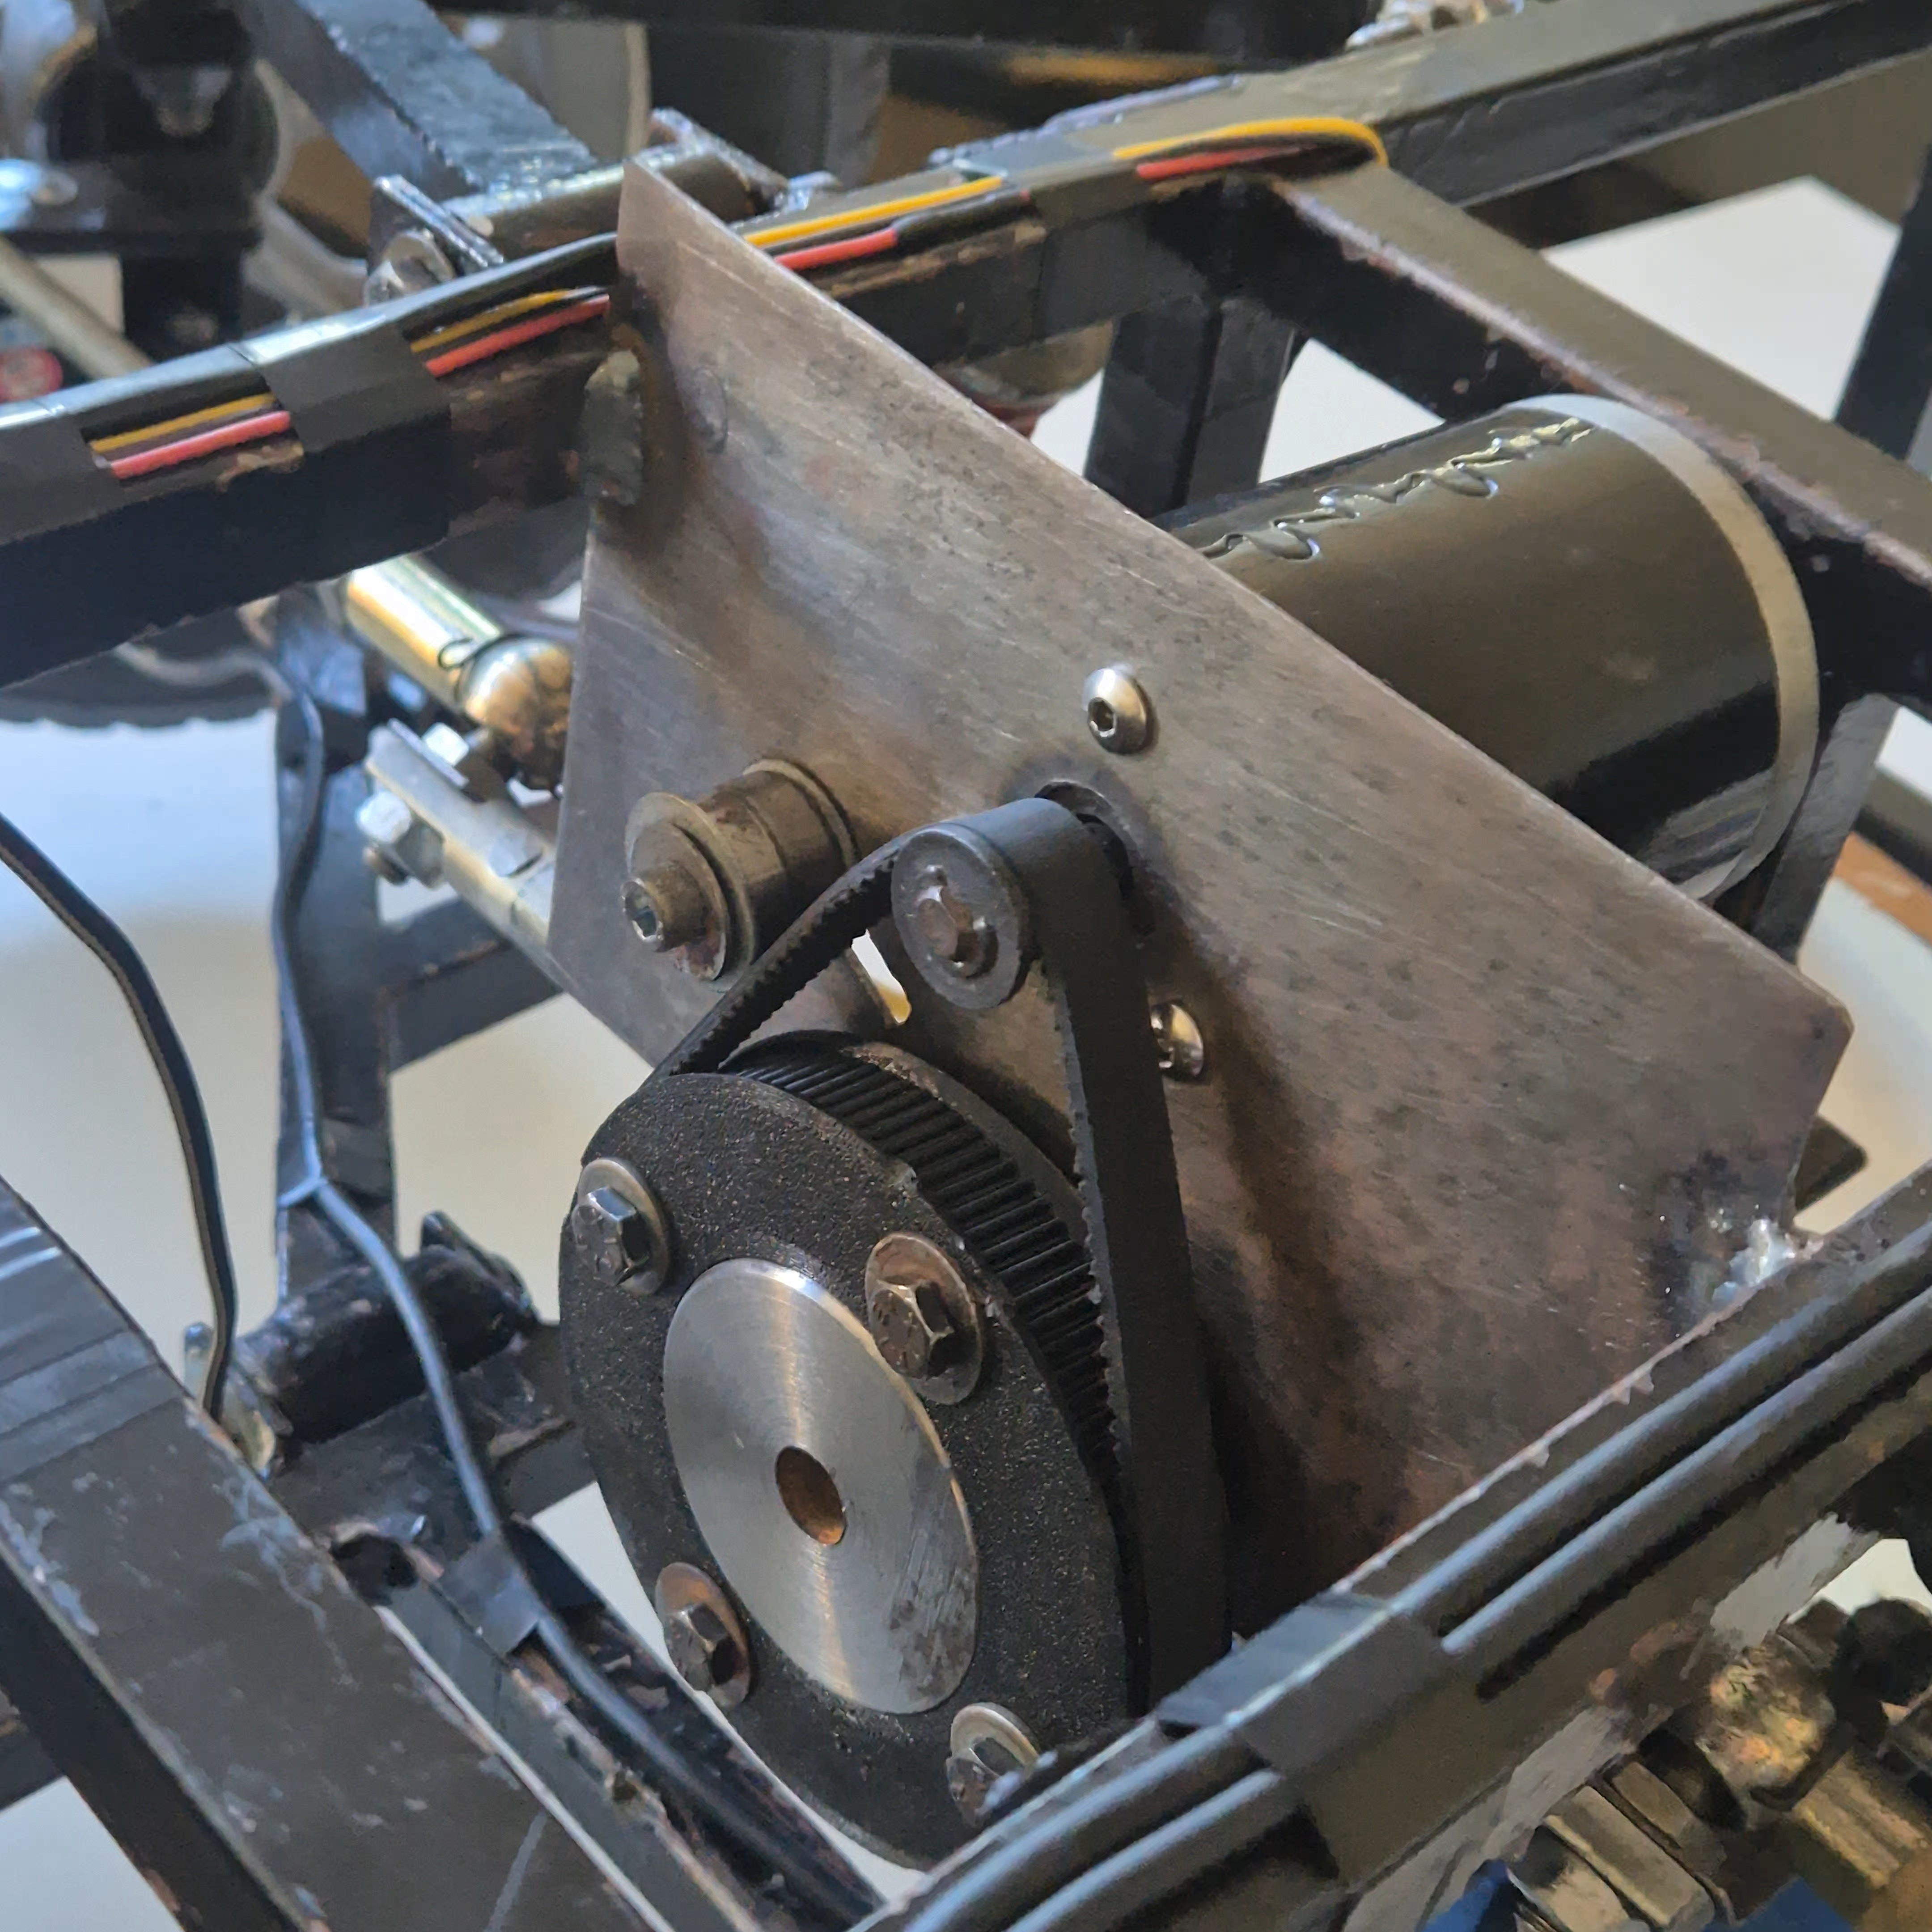
\includegraphics[width=0.72\columnwidth]{Imagens/Conjunto de esterçamento.jpg}
   \caption{Conjunto de esterçamento
    do VIDA. Fonte: Acervo do autor.}
    \label{fig:estercamento_vida}
\end{figure}


\subsection{Sistema Elétrico}

O sistema elétrico do VIDA passou por uma reformulação para atender às necessidades de alimentação, acionamento e integração dos componentes embarcados. A arquitetura implementada utiliza quatro baterias de 12 V, sendo três conectadas em série para formar um banco de 36 V, destinado aos circuitos de potência, e uma bateria independente de 12 V, responsável pela alimentação dos sistemas eletrônicos e periféricos.

A distribuição de energia foi organizada em um painel elétrico centralizado, que reúne os dispositivos de proteção, os conversores de tensão e os circuitos de comando. Os bancos de alimentação possuem entradas distintas no painel, buscando reduzir a interferência dos acionamentos de potência sobre os circuitos eletrônicos. O esquema elétrico completo do sistema de alimentação e distribuição de energia é apresentado no Apêndice~\ref{ap:esquema_eletrico}.

No circuito auxiliar, a tensão proveniente da bateria de 12 V é inicialmente elevada para 18 V por meio de um conversor CC-CC. Essa tensão é utilizada diretamente na alimentação do sensor LVDT e como entrada de um segundo estágio de regulação, responsável por fornecer uma tensão estabilizada de 12 V aos dispositivos periféricos. A partir dessa saída, um terceiro conversor reduz a tensão para 5 V, utilizada na alimentação dos componentes que operam nesse nível de tensão.

O circuito principal de 36 V alimenta os sistemas de potência e de comando. Parte dessa alimentação é convertida para 12 V, destinada aos dispositivos de operação, sinalização e acionamento dos relés auxiliares. O barramento de potência é interrompido por um relé principal normalmente aberto, cuja saída fornece 36 V ao sistema de tração e alimenta um conversor CC-CC, responsável por fornecer 24 V ao motor de esterçamento.

O painel dispõe de chave seccionadora geral, disjuntores de proteção, botões de acionamento, dispositivo de parada de emergência e sinalizadores luminosos. A lógica de comando utiliza relés auxiliares para controlar a habilitação do barramento de potência e disponibilizar um sinal lógico de 5 V aos sistemas de controle quando o veículo está habilitado.

A Figura~\ref{fig:painel_eletrico_vida} apresenta a implementação física do painel, destacando a organização dos conversores, dispositivos de proteção, relés e bornes de distribuição, bem como os elementos de comando instalados na porta. 

\begin{figure}[htb]
    \centering
    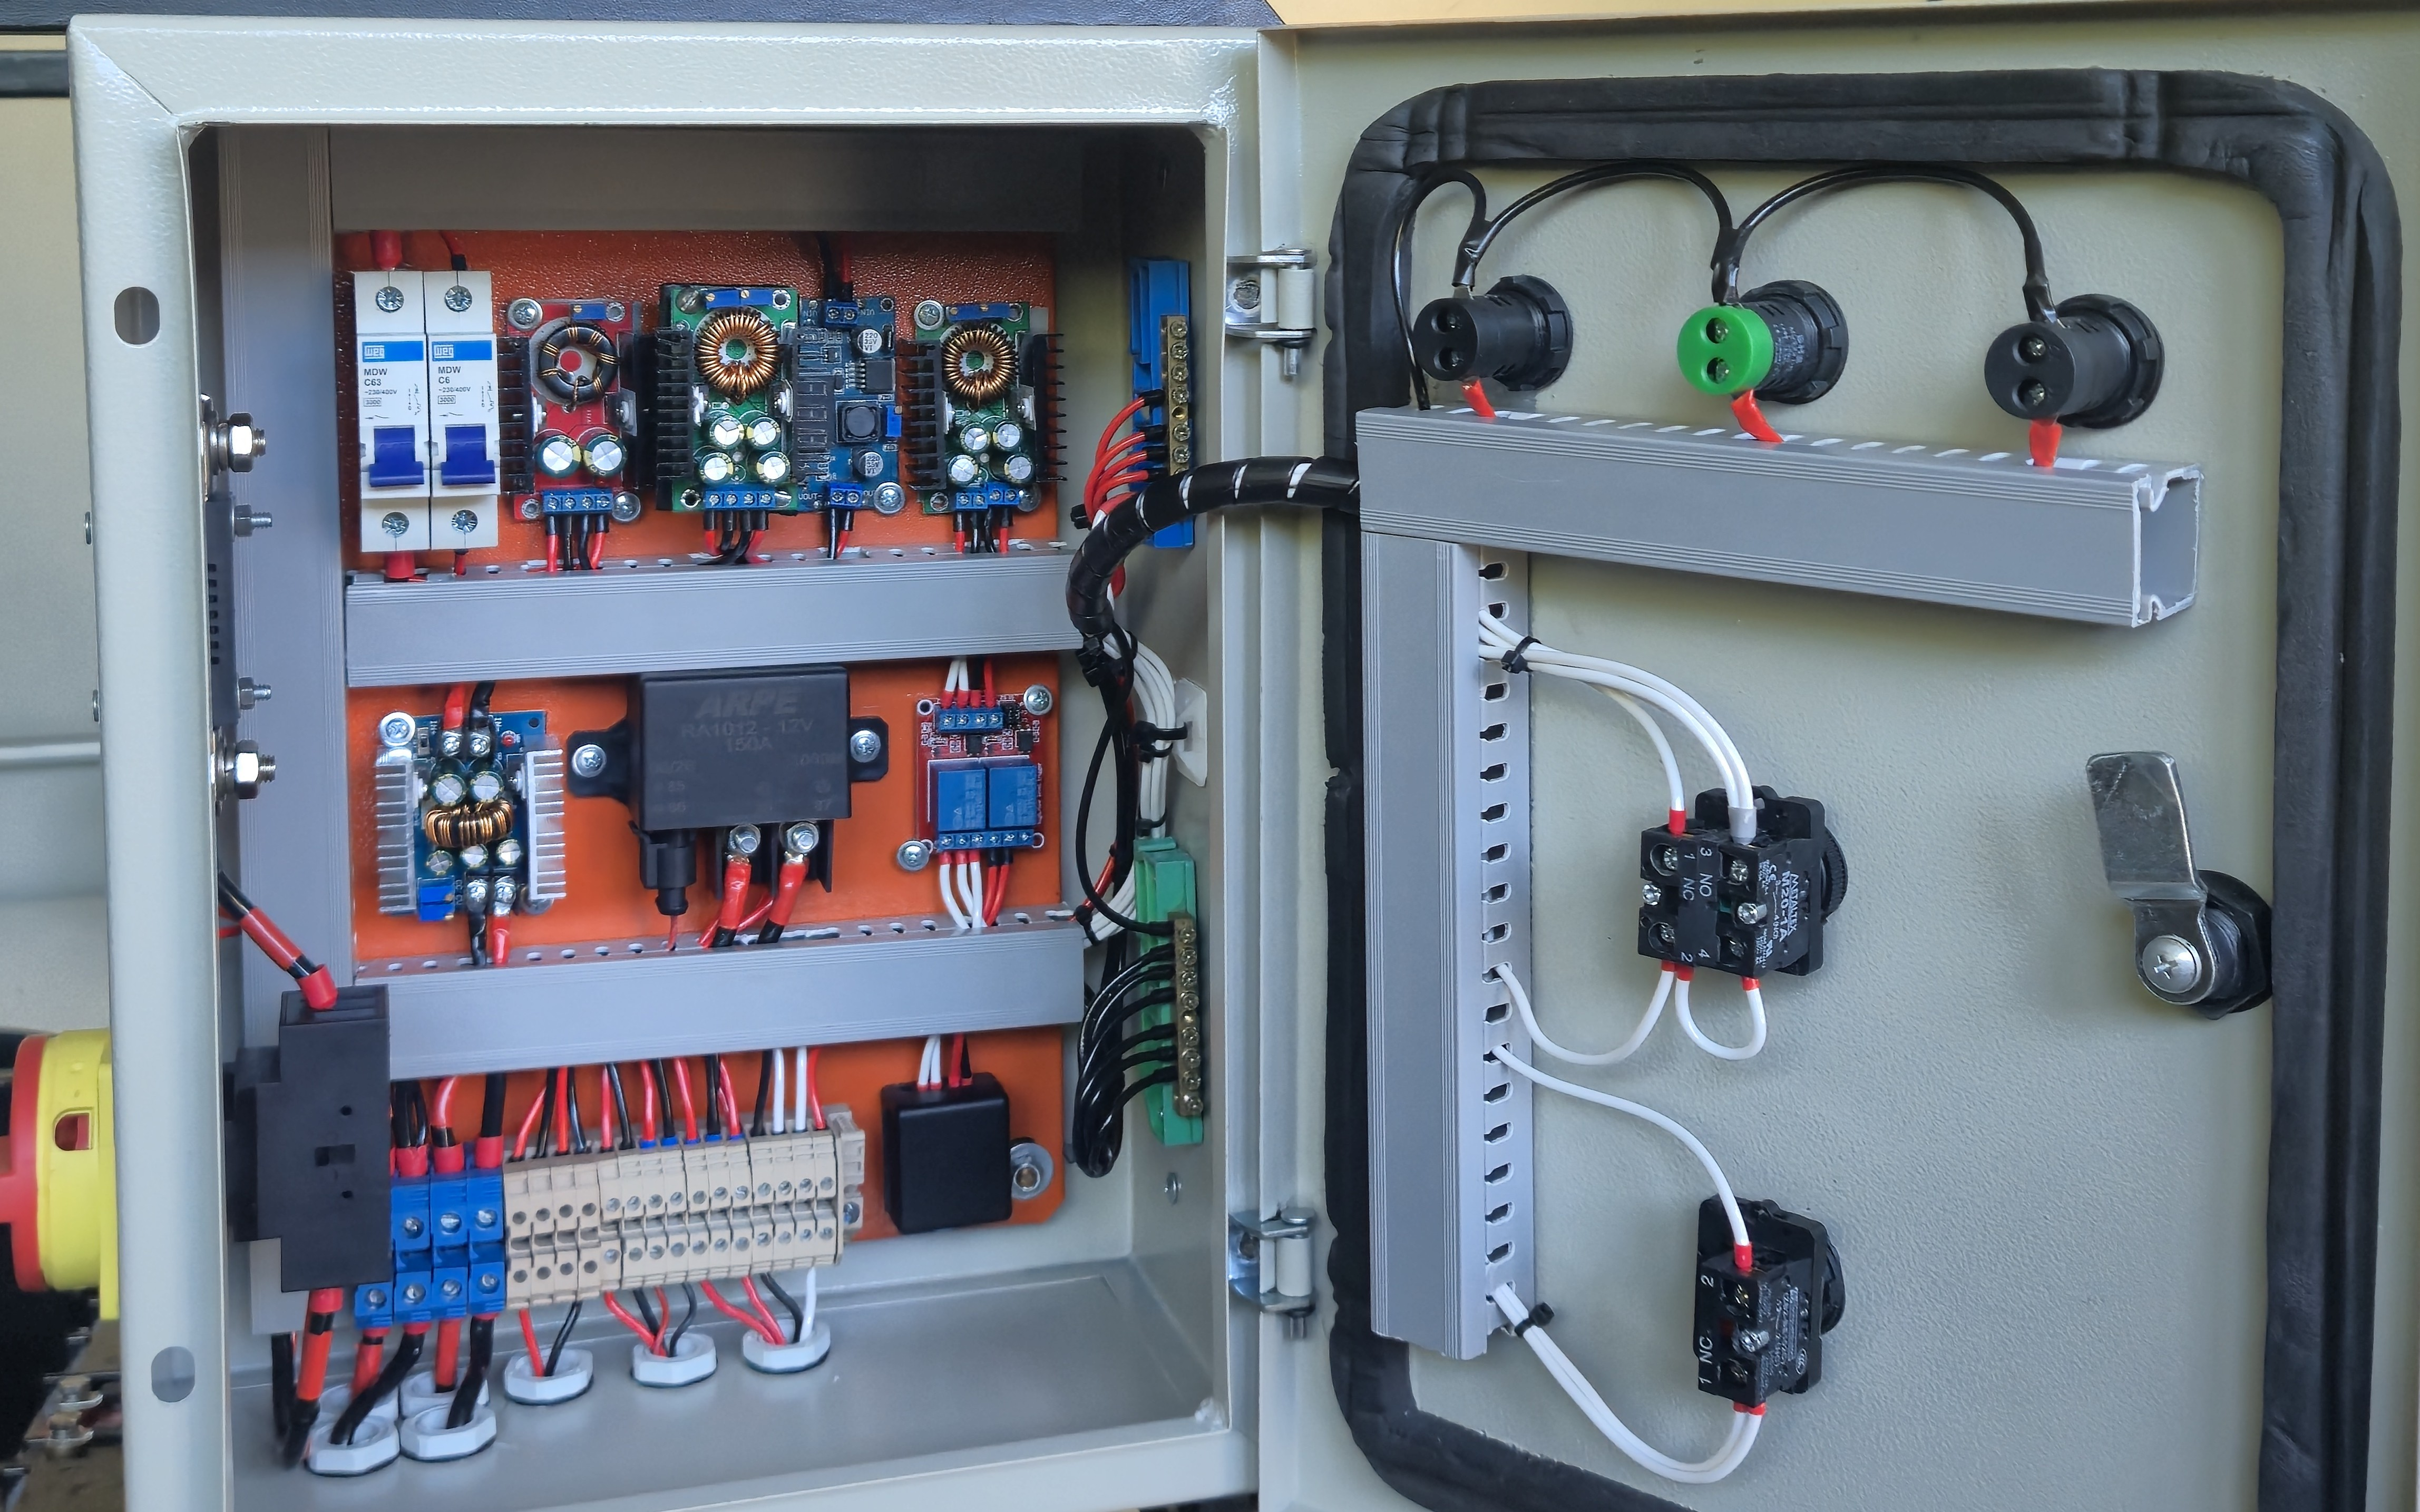
\includegraphics[width=0.85\columnwidth]{Imagens/Painel.jpg}
    \caption{Vista interna do painel elétrico do VIDA. Fonte: Acervo do autor.}
    \label{fig:painel_eletrico_vida}
\end{figure}


\subsection{Instrumentação e Sensoriamento}

A instrumentação do VIDA é composta por sensores destinados à aquisição de informações relacionadas ao movimento, à orientação e à localização do veículo. Para o desenvolvimento deste trabalho, foram utilizados três encoders incrementais, um sensor de deslocamento linear LVDT e um receptor GNSS com sensores inerciais integrados.

Os encoders incrementais são responsáveis pela medição da rotação das rodas, permitindo estimar o deslocamento e a velocidade longitudinal do veículo. Dois sensores estão instalados nas rodas dianteiras, enquanto o terceiro está instalado no eixo traseiro. Todos possuem dois canais de saída em quadratura, permitindo a identificação do sentido de rotação. A aquisição utiliza decodificação em quadratura completa, com resoluções configuradas de 720 contagens por revolução para os encoders dianteiros e 1440 para o traseiro.

O sensor LVDT (\textit{Linear Variable Differential Transformer}) é utilizado para medir o deslocamento linear do mecanismo de direção. Por meio de uma relação de calibração, essa medição permite determinar o ângulo de esterçamento das rodas dianteiras, fornecendo a realimentação necessária ao sistema de controle de direção.

Para o posicionamento global, utiliza-se o receptor GNSS u-blox ZED-F9R, que permite o emprego de correções RTK para obtenção de estimativas de posição de maior precisão. O dispositivo também integra sensores inerciais, incluindo um giroscópio, cujas informações de velocidade angular contribuem para a estimação da orientação do veículo.

A Tabela~\ref{tab:sensores_vida} apresenta um resumo dos principais sensores utilizados na plataforma.

\begin{table}[htb]
    \centering
    \caption{Instrumentação utilizada na plataforma VIDA.}
    \label{tab:sensores_vida}
    \small
    \begin{tabular}{lll}
        \hline
        \textbf{Dispositivo} &
        \textbf{Qtd.} &
        \textbf{Grandeza medida} \\
        \hline
        Encoder dianteiro & 2 & Rotação das rodas dianteiras \\
        Encoder traseiro & 1 & Rotação do eixo traseiro \\
        LVDT & 1 & Angulo de esterçamento \\
        GNSS ZED-F9R & 1 & Posição geográfica \\
        Giroscópio ZED-F9R & 1 & Velocidade angular \\
        \hline
    \end{tabular}
\end{table}